Zanim zostanie omówiona problematyka pracy, warto przywołać ważne definicje oraz fakty niezbędne do zrozumienia kolejnych rozdziałów. W oddzielnym podrozdziale skupiono się na testowaniu automatycznym: definicji, korzyściach płynących z jego zastosowania oraz mankamentach.


\section{Testowanie oprogramowania} \ 


\begin{df}
\textbf{Testowanie oprogramowania} (ang. \textit{software testing}) jest procesem związanym z zapewnieniem jakości oprogramowania, składający się z jego przygotowania i ewaluacji w celu stwierdzenia, czy spełnia określone wymagania oraz wykrywania defektów. \cite{roman} oraz \cite{myers}.

Proces ten składa się z dwóch ważnych pojęć:
\begin{itemize}
    \item \textbf{weryfikacji}, polegającej na ocenie, czy produkt spełnia określone warunki;
    \item \textbf{walidacji}, sprawdzającej poprawności procesu tworzenia produktu pod względem spełniania wymagań zamawiającego.
\end{itemize}

\end{df}

\begin{figure}[H]
\centering
\captionsetup{justification=centering}
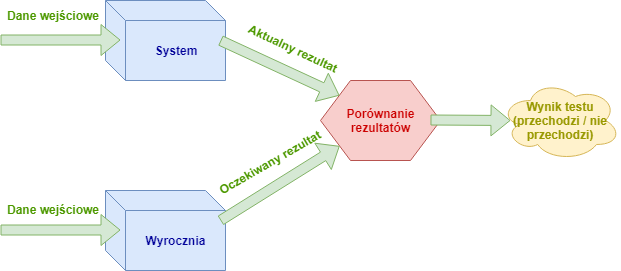
\includegraphics[width=1\textwidth]{Test.png}
\caption[Schemat procesu testowania]{\label{fig:proc}Schemat procesu testowania \\ źródło: \textit{opracowanie własne}}
\end{figure}

Wprowadzone zostają dane wejściowe zarówno dla testowanego systemu, jak i dla wyroczni, która jest odzwierciedleniem, jak powinien zachowywać się system. Po wykonaniu określonych czynności dokonuje się porównania oczekiwanego rezultatu z aktualnym. Jeżeli one różnią się między sobą, wtedy test wykrył defekt.

\section{Podziały testowania}

Uwzględnia się dwa niezależne od siebie podziały testów: 
\begin{itemize}
    \item \textbf{poziom}, odnoszący się do etapów wytwarzania oprogramowania.
    \item \textbf{typ}, klasyfikujący ze względu na cel testowania.
\end{itemize}
  Warto zwrócić uwagę, że każdy typ testu może być wykonany na każdym poziomie testowania, przykładowo testy systemowe mogą dotyczyć funkcjonalności systemu.

\noindent Wyróżniamy następujące poziomy testowania (\cite{roman} oraz \cite{smiglin}):
\begin{itemize}
    \item \textbf{testy jednostkowe} - sprawdzanie pojedynczego modułu bądź komponentu (np. klasy, funkcji) w izolacji od innych.
    \item \textbf{testy integracyjne} - zostaje przetestowana integracja między podanymi komponentami lub systemami.
    \item \textbf{testy systemowe} - wykonuje się je na już zintegrowanym oraz spójnym systemie i sprawdza się jego zgodność z wymaganiami.
    \item \textbf{testy akceptacyjne} - przeprowadza się je w celu akceptacji oprogramowania przez użytkownika lub klienta na środowisku produkcyjnym.
\end{itemize}

\noindent Testowanie możemy również podzielić ze względu na cel jego wykonywania (\cite{roman} oraz \cite{smiglin}):
\begin{itemize}
    \item \textbf{funkcjonalne (czarnoskrzynkowe)} - weryfikacja funkcjonalności produktu, to znaczy jakie są oczekiwane jego zachowania na określone działania użytkownika.
    \item \textbf{niefunkcjonalne} - wnikanie w to, jak działają komponenty. Inaczej, sprawdzamy cechy oprogramowania, takie jak efektywność, niezawodność, wydajność czy łatwość obsługi. 
    \item \textbf{białoskrzynkowe}, które jest oparte na wewnętrznej analizie struktury systemu; zapewnia, że wszystkie strukturalne elementy oprogramowania (np. linie kodu czy warunki logiczne w predykatach) zostały pokryte przez testy.
    \item \textbf{regresywne (regresyjne)} - ponowne przetestowanie oprogramowania  po dokonanym w nim zmianach dla upewnienia się, że nie powstały nowe błędy bądź nie ujawniły się w niezmodyfikowanych częściach produktu.
    \item \textbf{retestowanie} polegające na uruchomieniu przypadków testowych, które wcześniej wykryły defekty, aby sprawdzić, czy błędy zostały naprawione.
    \item \textbf{dymne} (ang. \textit{smoke testing}) - zawiera przypadki testowe pokrywające kluczowe funkcjonalności systemu lub komponentu w celu potwierdzenia ich działania, pomijając zagłębianie się w dalsze szczegóły.
\end{itemize}


Każdy proces podlega pewnym określonym zasadom. Nie inaczej jest w przypadku testowania - zaczerpnięte z \cite{istqb} siedem uniwersalnych zasad testowania:
\begin{enumerate}
    \item \textbf{Testowanie ujawnia usterki} - celem tego procesu jest udowodnienie, że oprogramowanie posiada defekty. Nawet jeżeli testowanie nie wykryło żadnych błędów, nie wynika stąd, że w ogóle nie występują w programie, ponieważ może istnieć w kodzie defekt, którego żaden dotychczasowy test nie znalazł.
    \item \textbf{Nie jest możliwe przetestowanie wszystkich możliwych kombinacji danych testowych} - głównie ze względu na czas i budżet przeznaczony na projekt. Należy się skupić tylko na tych przypadkach, które są najczęściej wykonywane oraz na tych z największym prawdopodobieństwem wystąpienia usterek.
    \item \textbf{Testowanie powinno odbywać się jak najwcześniej} - im we wcześniejszym etapie cyklu życia oprogramowania wykryje się defekt, tym szybciej i taniej da się go naprawić – co innego, jeżeli jest to błąd w specyfikacji czy przy pierwszej wersji oprogramowania, a co innego błąd znaleziony na produkcji.
    \item \textbf{Kumulacja błędów} - w testowaniu również obowiązuje zasada Pareto 80/20, mianowicie 80\% błędów znajduje się w 20\% modułów. Defekty “skupiają się” w jednym miejscu - biorąc pod uwagę ten fakt, w pierwszej kolejności należałoby je poddać testom. Jeżeli zna się dobrze oprogramowanie, można sprawnie znaleźć te części, w których jest największe ryzyko pojawienia się usterek. 
    \item \textbf{Paradoks pestycydów} - polega on na tym, że jeżeli spryskuje się pole tym samym środkiem owadobójczym, to po pewnym czasie pluskwy na niego się uodpornią i środek przestaje na nich działać. To samo zjawisko występuje w testowaniu: gdy wykonujemy niemodyfikowane testy, przestają one skutecznie wykrywać błędy w oprogramowaniu. Powinno się sprawdzać regularnie oraz aktualizować istniejące testy, żeby zapobiec temu zjawisku. Dodatkowo, należy także dodawać nowe testy badające pozostałe części oprogramowania tak, żeby znalazły kolejne defekty.
    \item \textbf{Testowanie jest zależne od kontekstu} - Nie da się dostosować tylko jednego procesu testowania do projektu, ponieważ do każdego z nich trzeba zastosować inne techniki, dopasować inne poziomy czy typy testów. Inaczej się sprawdza aplikację webową, a inaczej mobilną, tak samo, przykładowo, system bankowy będzie wymagał odrębnego podejścia do testowania niż system telekomunikacyjny. 
    \item \textbf{Fałszywe przekonanie o braku defektów} - Dla klienta najważniejsze jest to, aby oprogramowanie spełniało określone przez niego wymagania, nawet jeżeli system zawiera błędy - póki one nie wpływają na funkcjonowanie programu, cel jest osiągnięty. 
\end{enumerate}

\section{Przypadek testowy a scenariusz testowy} \ 

Często pojawiającymi się pojęciami w testowaniu są te podane w tytule podrozdziału. Zostaną one wyjaśnione oraz zostanie pokazana różnica między nimi.

\begin{df}
\textbf{Przypadek testowy} (ang. \textit{test case}) jest zbiorem danych wejściowych, warunków wstępnych, oczekiwanych rezultatów i warunków kończących wykonanie testu. \cite{przypadek}
\end{df}

\begin{prz}
Rozważony zostaje przypadek testowy dla kodów USSD (służące do komunikacji między telefonem komórkowym a elementami sieci komórkowych) - sprawdzenie salda abonenta (przykładowo kod ten jest równy $*123\#$). 

\noindent \textbf{Przypadek:} sprawdzenie salda abonenta za pomocą kodu USSD.

\noindent \textbf{Warunki wstępne:} włączony i działający telefon komórkowy z testową kartą prepaid. Nie może być uruchomiony żaden kod USSD.

\noindent \textbf{Kroki testowe:} 
\begin{enumerate}
    \item Kliknij w telefonie przycisk do dzwonienia.
    \item Wpisz $*123\#$.
    \item Zatwierdź, klikając przycisk do dzwonienia. Odczekaj do momentu pojawienia się wiadomości (maksimum 5 sekund).
\end{enumerate}

\noindent \textbf{Oczekiwany rezultat:} Pojawienie się na ekranie komunikatu: ``Stan Twojego konta: X zł".

\noindent \textbf{Warunki końcowe:} Na ekranie wyświetla się prawidłowy stan konta abonenta.

\end{prz}




\begin{df}
\textbf{Scenariusz testowy} lub \textbf{skrypt testowy} (ang. \textit{test scenario} lub \textit{test script}) to procedura określająca ciąg akcji, dzięki którym można wykonać test. \cite{roman} oraz \cite{ieee}
\end{df}

\begin{prz}
Odnosząc się do przykładu 2.2.3., jednym ze scenariuszy testowych do sprawdzenia kodów USSD mógłby wyglądać tak:

\begin{enumerate}
    \item Sprawdzenie salda abonenta.
    \item Wpisanie kodu nieistniejącego - wyświetlenie się komunikatu o błędnym kodzie. 
    \item Ponowne sprawdzenie stanu konta, czy jest taki sam, jak na samym początku.
    \item Napisanie SMSa, które kosztuje $x$ zł.
    \item Sprawdzenie czy saldo zostało pomniejszone o $x$ zł.
\end{enumerate}

\end{prz}

Można zauważyć między innymi po ostatnim przykładzie, że tak naprawdę scenariusz testowy składa się z wielu przypadków testowych.

\section{Pozostałe definicje} \ 

Zostaną tutaj wymienione pozostałe definicje nie pasujące do poprzednich podrozdziałów, które będą się pojawiać w pracy.

\begin{df}
\textbf{Aplikacja internetowa (webowa)} (ang. \textit{web application}) jest programem komputerowym pracującym na serwerze i komunikującym się za pomocą sieci komputerowej z hostem użytkownika komputera używając przeglądarki internetowej użytkownika. Przy pracy musi pośredniczyć serwer WWW. \cite{webapp}
\end{df}

\begin{df}
\textbf{Środowisko testowe} (ang. \textit{test environment}) jest środowiskiem, w którego skład wchodzi sprzęt, oprogramowanie oraz inne elementy potrzebne do wykonania testów. \cite{roman} oraz \cite{ieee}
\end{df}

\begin{df}
\textbf{Testowanie wydajnościowe} (ang. \textit{performance testing}) ma na celu zbadanie oraz porównanie czasu odpowiedzi przejścia pojedynczego przez system lub aplikację z odpowiedzią wielu użytkowników, aby sprawdzić, czy poszczególne akcje są wykonywane przez niego w akceptowalnym czasie. \cite{roman}
\end{df}

\begin{df}
\textbf{Testowanie obciążeniowe} (ang. \textit{load testing}) polega na zbadaniu, jak wiele zapytań jest w stanie obsłużyć system w danym przedziale czasowym przy utrzymaniu dużej liczby jednocześnie działających użytkowników lub transakcji. \cite{roman}
\end{df}

